\documentclass[class=article, crop=false]{standalone}
\usepackage[fleqn]{amsmath}
\usepackage{amssymb}
\usepackage{graphicx}
\graphicspath{ {../images/} }
\begin{document}

\section*{Definition}
$\mathbb{R}$ is the set of real numbers which we have been using before. This can be thought of as a straight number line. The complex numbers ($\mathbb{C}$) can be thought of as a plane of numbers of which the real numbers is one axis. $\mathbb{R} \subset \mathbb{C}$. \\

$x^2 = -1$ has no real roots. We can imagine that this equation has a root. We define $i$ such that $i^2 = -1$. $i$ is imaginary. \\

Complex numbers are made up of the form $a+bi$, $a,b \in \mathbb{R}$. We often use $z$ to represent complex numbers rather than $x$. \\

$z = a+bi \Rightarrow \operatorname{Re}(z)=a, \operatorname{Im}(z)=b$ \\

We say two complex numbers are equal if both the real and imaginary parts are the same. We also assume that the same rules of algebra apply to complex numbers as real numbers. We can not find roots for any polynomial with real coefficients. 

\subsubsection*{Example 1}
\begin{align*}
& x^2 + 2x + 8 = 0 \\
\Rightarrow & x = \frac{-2 \pm \sqrt{4-32}}{2} \\
& = \frac{-2 \pm \sqrt{4} \sqrt{-7}}{2} \\
& = -1 \pm \sqrt{7}i \\
\end{align*}

The conjugate of a complex number $z = a+bi$ is $z^* = a-bi$. This is useful for eliminating a complex denominator on a fraction. 
\subsubsection*{Example 2}
\begin{align*}
\frac{3 + 5i}{2-3i} & = \frac{3 + 5i}{2-3i} * \frac{2+3i}{2+3i} \\
& = \frac{6 + 19i + 15i^2}{4-9i^2} \\
& = \frac{-9 + 19i}{13} \text{ or } \frac{-9}{13} + \frac{19}{13}i \\
\end{align*}

\section*{The Argand Diagram}
The Argand diagram is a graphical representation of $\mathbb{C}$, much like a number line is used to represent $\mathbb{R}$. \\
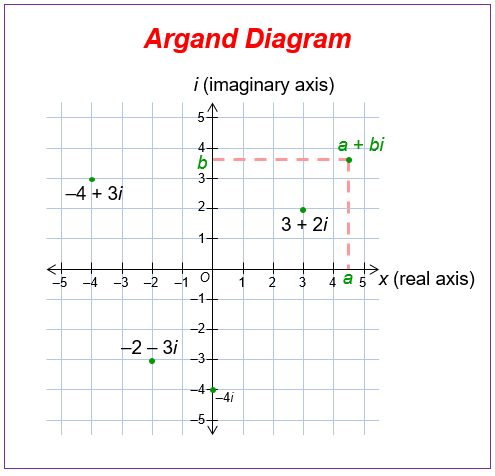
\includegraphics[scale=0.5]{argandDiagram} \\

\section*{Modulus and Argument}
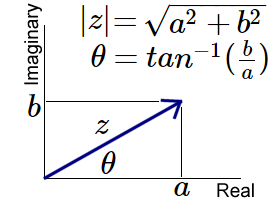
\includegraphics[scale=0.5]{ModulusandArgument} \\
The argument of z (written $\arg z$) is the angle from the real axis. The principle argument is $-\pi < \arg z \leqslant \pi$. There may be two solutions so it is best to think about where the point would be on the Argand diagram to find which one is correct. \\

The modulus of z (written $|z|$) is the distance from $(0,0)$ to $(a,b)$ and can be used to compare the size of complex numbers. \\

\subsection*{Modulus - Argument Form}
Complex numbers can be thought of as an angle and distance from the origin. \\
$|z| = r$, $\arg z = \theta$ $\Rightarrow$ $z = r(\cos \theta + i \sin \theta)$ \\
$\operatorname{Re}(z) = |z| \cos \arg z$, $\operatorname{Im}(z) = |z| \sin \arg z$ \\
Modulus - Argument Form is useful as it makes multiplication of complex numbers easier and allows us to think of them as transforms. \\
\begin{align*}
z_1 & = r_1(\cos \theta_1 + i \sin \theta_1) \\
z_2 & = r_2(\cos \theta_2 + i \sin \theta_2) \\
\Rightarrow z_1 z_2 & = r_1(\cos \theta_1 + i \sin \theta_1) \times r_2(\cos \theta_2 + i \sin \theta_2) \\
& = r_1 r_2(\cos \theta_1 \cos \theta_2 - \sin \theta_1 \sin \theta_2 + i \cos \theta_1 \sin \theta_2 + i \cos \theta_2 \sin \theta_1) \\
& = r_1 r_2(\cos(\theta_1 + \theta_2) + i \sin(\theta_1 + \theta_2)) \\
\therefore & |z_1 z_2| = |z_1| \times |z_2| \\
& \arg(z_1 z_2) = \arg z_1 + \arg z_2 \\
\end{align*}
In the context of the Argand diagram multiplying by a complex number is equivalent to:
\begin{itemize}
	\item Rotation by $\arg z$ around $(0,0)$
	\item Scale by $|z|$ about $(0,0)$
\end{itemize} 
Dividing is equivalent to:
\begin{itemize}
	\item Rotation by $- \arg z$ around $(0,0)$
	\item Scale by $\frac{1}{|z|}$ about $(0,0)$
\end{itemize} 
\end{document}